%(BEGIN_QUESTION)
% Copyright 2009, Tony R. Kuphaldt, released under the Creative Commons Attribution License (v 1.0)
% This means you may do almost anything with this work of mine, so long as you give me proper credit

A flow measurement loop has a problem, and you are called to diagnose it.  According to the loop sheet, the transmitter is supposed to be configured with square-root characterization, while the indicator is supposed to be linear:

$$\includegraphics[width=15.5cm]{i04053x01.eps}$$

The DP transmitter's range is 0 to 100 inches water column, and the indicator's range is 0 to 250 GPM.  Disconnecting the transmitter from the orifice plate impulse tubes, you connect a hand pump and precision test gauge to the ``high'' input port and proceed to apply the following pressures to the transmitter, while calling a fellow technician over a hand-held radio to read what the indicator says, and watching the display of a digital multimeter as it measures the transmitter's output current.  The result is this table of values:

% No blank lines allowed between lines of an \halign structure!
% I use comments (%) instead, so that TeX doesn't choke.

$$\vbox{\offinterlineskip
\halign{\strut
\vrule \quad\hfil # \ \hfil & 
\vrule \quad\hfil # \ \hfil & 
\vrule \quad\hfil # \ \hfil \vrule \cr
\noalign{\hrule}
%
% First row
Applied pressure & Current signal & Indicator display \cr
%
\noalign{\hrule}
%
% Another row
0 "W.C. & 5.6 mA & 25.0 GPM \cr
%
\noalign{\hrule}
%
% Another row
40 "W.C. & 14.2 mA & 159.4 GPM \cr
%
\noalign{\hrule}
%
% Another row
80 "W.C. & 18.4 mA & 225.0 GPM \cr
%
\noalign{\hrule}
%
% Another row
100 "W.C. & 20.08 mA & 251.3 GPM \cr
%
\noalign{\hrule}
} % End of \halign 
}$$ % End of \vbox

Determine the location of the problem in this loop, based on these measurements.  Also, explain why it is very helpful in your diagnosis to have the meter measurements of signal current, rather than just know what the indicator reads for each of the applied pressures.

\vskip 20pt \vbox{\hrule \hbox{\strut \vrule{} {\bf Suggestions for Socratic discussion} \vrule} \hrule}

\begin{itemize}
\item{} A valuable principle to apply in a diagnostic scenario such as this is {\it correspondence}: identifying which values agree with each other: applied pressure, current signal, and indicator.  Explain how a check of correspondence tells us which instrument is at fault in this system.
\item{} Describe the proper procedure for isolating this transmitter from the process line prior to applying test pressures to check its calibration.
\item{} Supposing this was a flow {\it control} loop with a PID controller sensing the flow rate and adjusting a control valve's position in response, what would we have to do to the controller before proceeding with the hand pump test in a live process?  If we did not properly configure the controller prior to this test, how would our hand pump test affect the working loop as it tried to stabilize flow at setpoint?
\end{itemize}

\underbar{file i04053}
%(END_QUESTION)





%(BEGIN_ANSWER)

%(END_ANSWER)





%(BEGIN_NOTES)

The problem is in the transmitter's sensor (i.e. a ``sensor trim'' error): it has a +1 "W.C. zero-shift (i.e. it ``thinks'' the applied pressure is 1 "W.C. greater than it actually is).  We can tell that the calibration error lies before the square-root characterization and not after due to the nonlinearity of the error: we're off by 1.6 mA at the LRV, off by 0.089 mA at 80\%, and only off by 0.08 mA at the URV.  If the error were linear, it would have to lie somewhere after the square-root calculation.

\vskip 10pt

Having measurements of transmitter current is extremely helpful because it gives us data we may use to independently assess the calibration of the transmitter versus the calibration of the indicator.  Without this ``measurement in the middle,'' the transmitter and indicator act as a single instrument with one input and one output, making it difficult to discern which half of the loop has the problem.

%INDEX% Measurement, flow: troubleshooting

%(END_NOTES)


